\section{結果}

湯気のシミュレーションの結果を図\ref{result}に示す。
実装では底面に一様な温度、水蒸気量を定義した結果である。
レンダリングには\cite{smoke3d}にある独自のレンダリングモジュールを用いた。
提案した手法を用いることで湯気の発生と消滅に近い映像を出力するできることを確認した。

\begin{figure}[htbp]
 \begin{minipage}{0.33\hsize}
  \begin{center}
   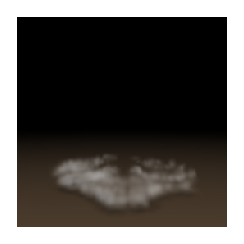
\includegraphics[width=40mm]{img/render_20.bmp}
  \end{center}
  \label{fig:one}
 \end{minipage}
 \begin{minipage}{0.33\hsize}
 \begin{center}
  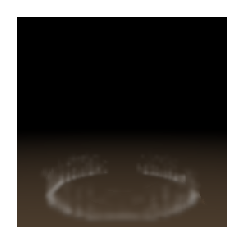
\includegraphics[width=40mm]{img/render_30.bmp}
 \end{center}
  \label{fig:two}
 \end{minipage}
 \begin{minipage}{0.33\hsize}
 \begin{center}
  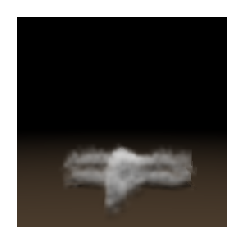
\includegraphics[width=40mm]{img/render_40.bmp}
 \end{center}
  \label{fig:three}
 \end{minipage}
\end{figure}

\begin{figure}[htbp]
 \begin{minipage}{0.33\hsize}
  \begin{center}
   
\includegraphics[width=40mm]{img/render_50.bmp}
  \end{center}
  \label{fig:four}
 \end{minipage}
 \begin{minipage}{0.33\hsize}
 \begin{center}
  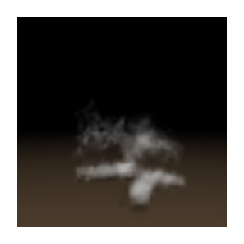
\includegraphics[width=40mm]{img/render_60.bmp}
 \end{center}
  \label{fig:five}
 \end{minipage}
 \begin{minipage}{0.33\hsize}
 \begin{center}
  \includegraphics[width=40mm]{img/render_70.bmp}
 \end{center}
  \label{fig:six}
 \end{minipage}
\end{figure}

\begin{figure}[htbp]
 \begin{minipage}{0.33\hsize}
  \begin{center}
   
\includegraphics[width=40mm]{img/render_80.bmp}
  \end{center}
  \label{fig:seven}
 \end{minipage}
 \begin{minipage}{0.33\hsize}
 \begin{center}
  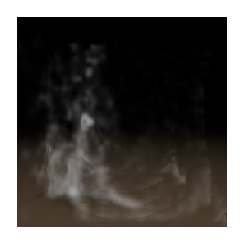
\includegraphics[width=40mm]{img/render_90.bmp}
 \end{center}
  \label{fig:eight}
 \end{minipage}
 \begin{minipage}{0.33\hsize}
 \begin{center}
  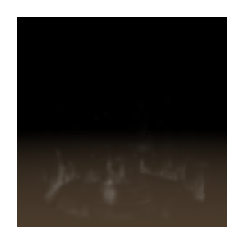
\includegraphics[width=40mm]{img/render_100.bmp}
 \end{center}
  \label{fig:nine}
 \end{minipage}
 \caption{湯気のシミュレーション結果}
 \label{result}
\end{figure}